
\documentclass[runningheads]{cl2emult}

\usepackage{makeidx}  % allows index generation
\usepackage{graphicx} % standard LaTeX graphics tool
                      % for including eps-figure files
\usepackage{subeqnar} % subnumbers individual equations
                      % within an array
\usepackage{multicol} % used for the two-column index
\usepackage{cropmark} % cropmarks for pages without
                      % pagenumbers
\usepackage{math}     % placeholder for figures
\usepackage{amssymb}     % placeholder for figures
\usepackage{subfigure} % subfigures in one figure

%\usepackage{algorithm2e}
\usepackage[ruled,algonl]{algorithm2e}
%\setlength{\algomargin}{2.1em}
\dontprintsemicolon
\SetInd{0.5em}{1em}
\SetKwFor{Forall}{forall}{do}{od}
\SetKwFor{WhileDo}{while}{do}{od}
\SetKw{Let}{let}

\makeindex            % used for the subject index
                      % please use the style sprmidx.sty with
                      % your makeindex program

%upright Greek letters (example below: upright "mu")
\newcommand{\euler}[1]{{\usefont{U}{eur}{m}{n}#1}}
\newcommand{\eulerbold}[1]{{\usefont{U}{eur}{b}{n}#1}}
\newcommand{\umu}{\mbox{\euler{\char22}}}
\newcommand{\umub}{\mbox{\eulerbold{\char22}}}
\newcommand{\url}[1]{{\small{\tt #1}}}

%%%%%%%%%%%%%%%%%%%%%%%%%%%%%%%%%%%%%%%%%%%%%%%%%%%%%%%%%%%%%

%OPTIONAL%%%%%%%%%%%%%%%%%%%%%%%%%%%%%%%%%%%%%%%%%%%%%%%%%%%%
%
%\usepackage{amstex}   % useful for coding complex math
%\mathindent\parindent % needed in case "Amstex" is used
%
%%%%%%%%%%%%%%%%%%%%%%%%%%%%%%%%%%%%%%%%%%%%%%%%%%%%%%%%%%%%%

%AUTHOR_STYLES_AND_DEFINITIONS%%%%%%%%%%%%%%%%%%%%%%%%%%%%%%%
%
%Please reduce your own definitions and macros to an absolute
%minimum since otherwise the editor will find it rather
%strenuous to compile all individual contributions to a
%single book file
%
%%%%%%%%%%%%%%%%%%%%%%%%%%%%%%%%%%%%%%%%%%%%%%%%%%%%%%%%%%%%%

\begin{document}
%
\title*{The WilmaScope 3D Graph Visualisation System}
%
%
\toctitle{WilmaScope}
% allows explicit linebreak for the table of content
%
%
\titlerunning{WilmaScope}
% allows abbreviation of title, if the full title is too long
% to fit in the running head
%
\author{Tim Dwyer\inst{1}
\and Peter Eckersley\inst{2}
}
%
\authorrunning{Tim Dwyer and Peter Eckersley}
% if there are more than two authors,
% please abbreviate author list for running head
%
%
\institute{School of Information Technologies,
     Madsen Building F09,
     University of Sydney,
     NSW 2006,
     Australia.
		 E-mail: \url{dwyer@cs.usyd.edu.au}
\and Department of Computer Science \& Software Engineering,
     University of Melbourne,
     Victoria 3010,
     Australia.
		 E-mail: \url{pde@cs.mu.oz.au}}

\maketitle              % typesets the title of the contribution



%\begin{abstract}
%The abstract\index{abstract} should summarize the contents of the paper
%in at least 70 and at most 150 words; neither too long
%nor too short but to the point!
%\end{abstract}

\section{Introduction}\label{sec:intro}

\subsection{Witty Survey Subsection}
{\em survey previous stuff.}

\subsection{The Motivation for WilmaScope}
\label{motivation}

Despite, or perhaps because of, the extensive research literature on graph
drawing techniques, there is a lack of state-of-the-art, general-purpose
visualisation systems, particularly for application to 3-dimensional
embeddings.

Graph drawing problems are, of course, exsitent within an enourmous range of
fields; a key motivation for creating a general purpose 3D visualisation
system is to provide easy-to-use components which can be employed by future
software across these application domains.

Within the graph drawing community itself, a system may also aspire to 
streamline, elucidate and beautify the work of algorithm design, comparison
and optimisation.  Achieving these benefits requires software which is
flexible, interactive and easily extensible.

In order to provide these benefits as widely as possible, and to guarantee
an enthusiastic culture of user participation, a serious graph visualisation
system should also be {\em Free Software}\cite{stallman92why}.

In this chapter, we describe WilmaScope (or ``Wilma'', for short), a
sophisticated graph visualisation infrastructure, which attempts to meet
these goals.  In Section~\ref{sec:design}, we describe the Wilma
architecture, modular subsystems, and facilities for control by human users
and other software.  Section~\ref{sec:results} we demonstrate Wilma in
action, with examples of graphical results, domain specific applications and
feedback from users.  Finally, Section~\ref{sec:conclusions} reviews Wilma's
contribution and identifies directions for future development.

\section{Design}\label{sec:design}
\subsection{High Level Architecture}
Conceived as a research project with open ended goals, Wilma was
designed to be as flexible and extensible as possible.  The intention
was to allow different components, such as new visual representations
for graph elements, interfaces (either graphical user interfaces or
remote programming interfaces) and different 
layout algorithm implementations to be added or removed easily.
Therefore the design needed to decouple these components as much as
possible so that altering one component would have minimal impact on
the other components.

To achieve this we began by exploring the well known Model-View-Controller
architecture (MVC) \cite{gamma94design}.  In an MVC architecture the Model is the core
of the application, the data and algorithms that automatically modify
the data.  The View is a user interface which displays information
about the model to the user.  The Controller is a separate user
interface that provides methods for the user to manipulate the
application, ie to control the Model.  Each components reference to
the other components is via a carefully defined interface which should
not require change one of the components is modified in some way.  The
standard data flow diagram for the MVC architecture is shown in Figure
\ref{fig-mvc}.

\begin{figure}[h]
  \centering
  \subfigure[MVC Architecture]{
    \label{fig-mvc}
    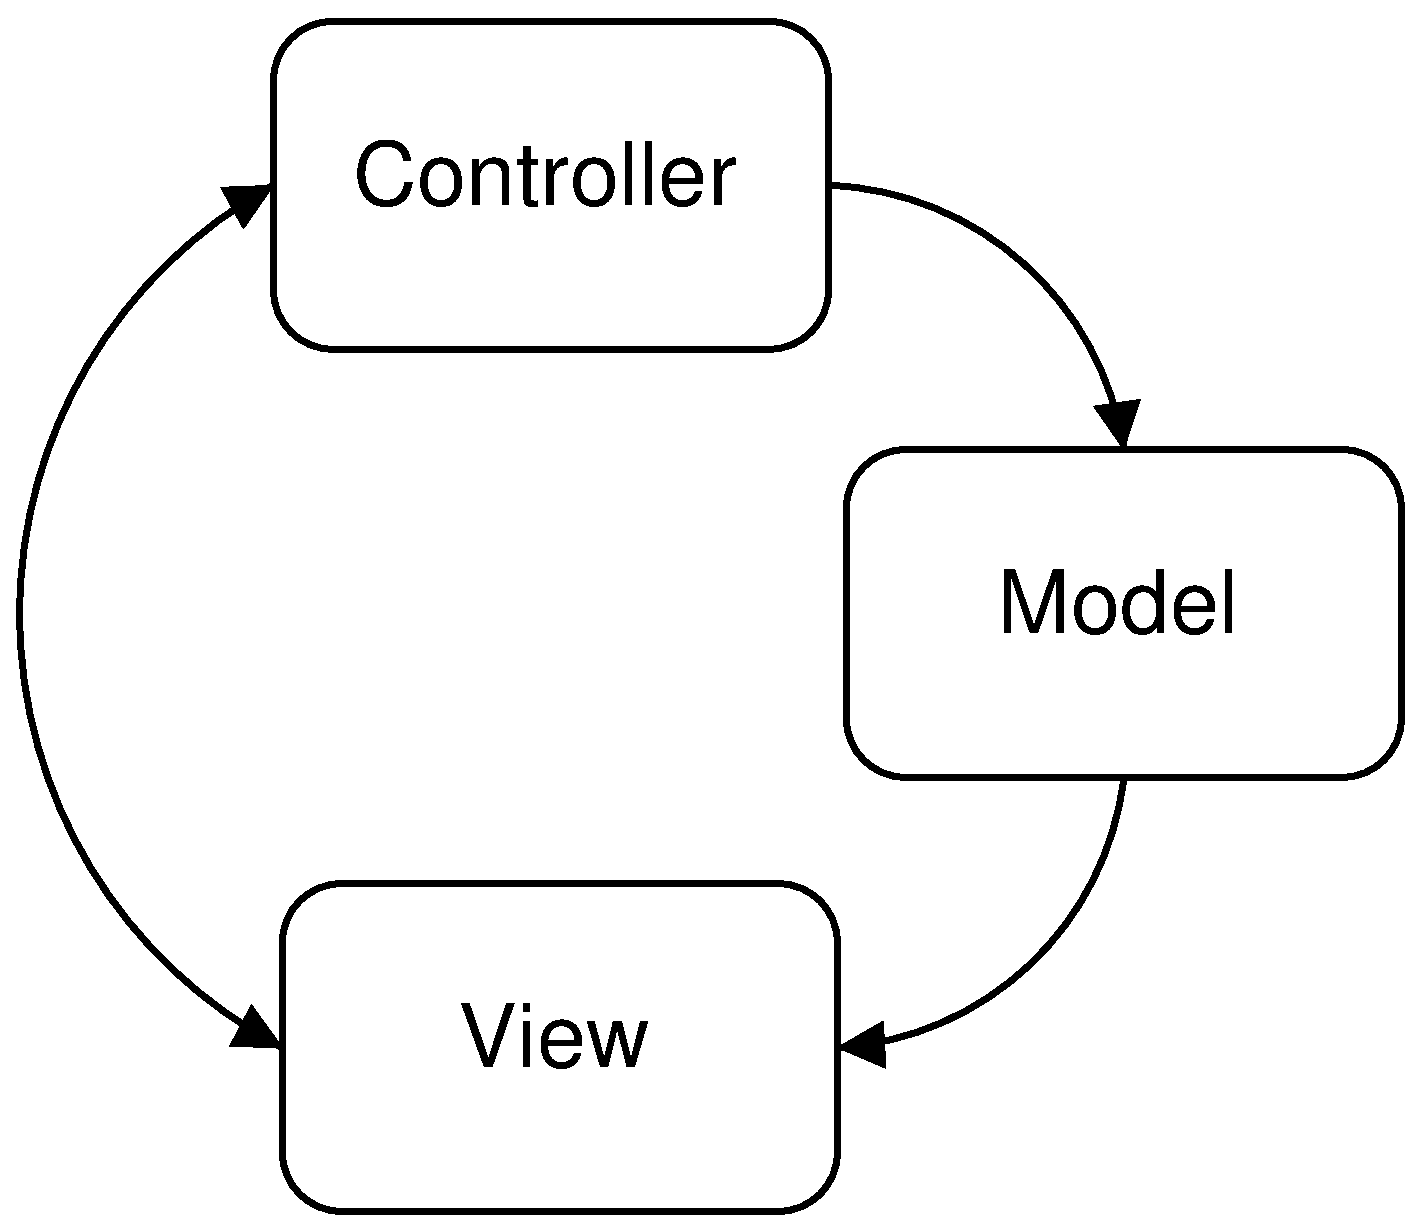
\includegraphics[width=0.4\textwidth]{figures/mvc.eps}}
  \subfigure[Wilma Architecture]{
    \label{fig-wilmamvc}
    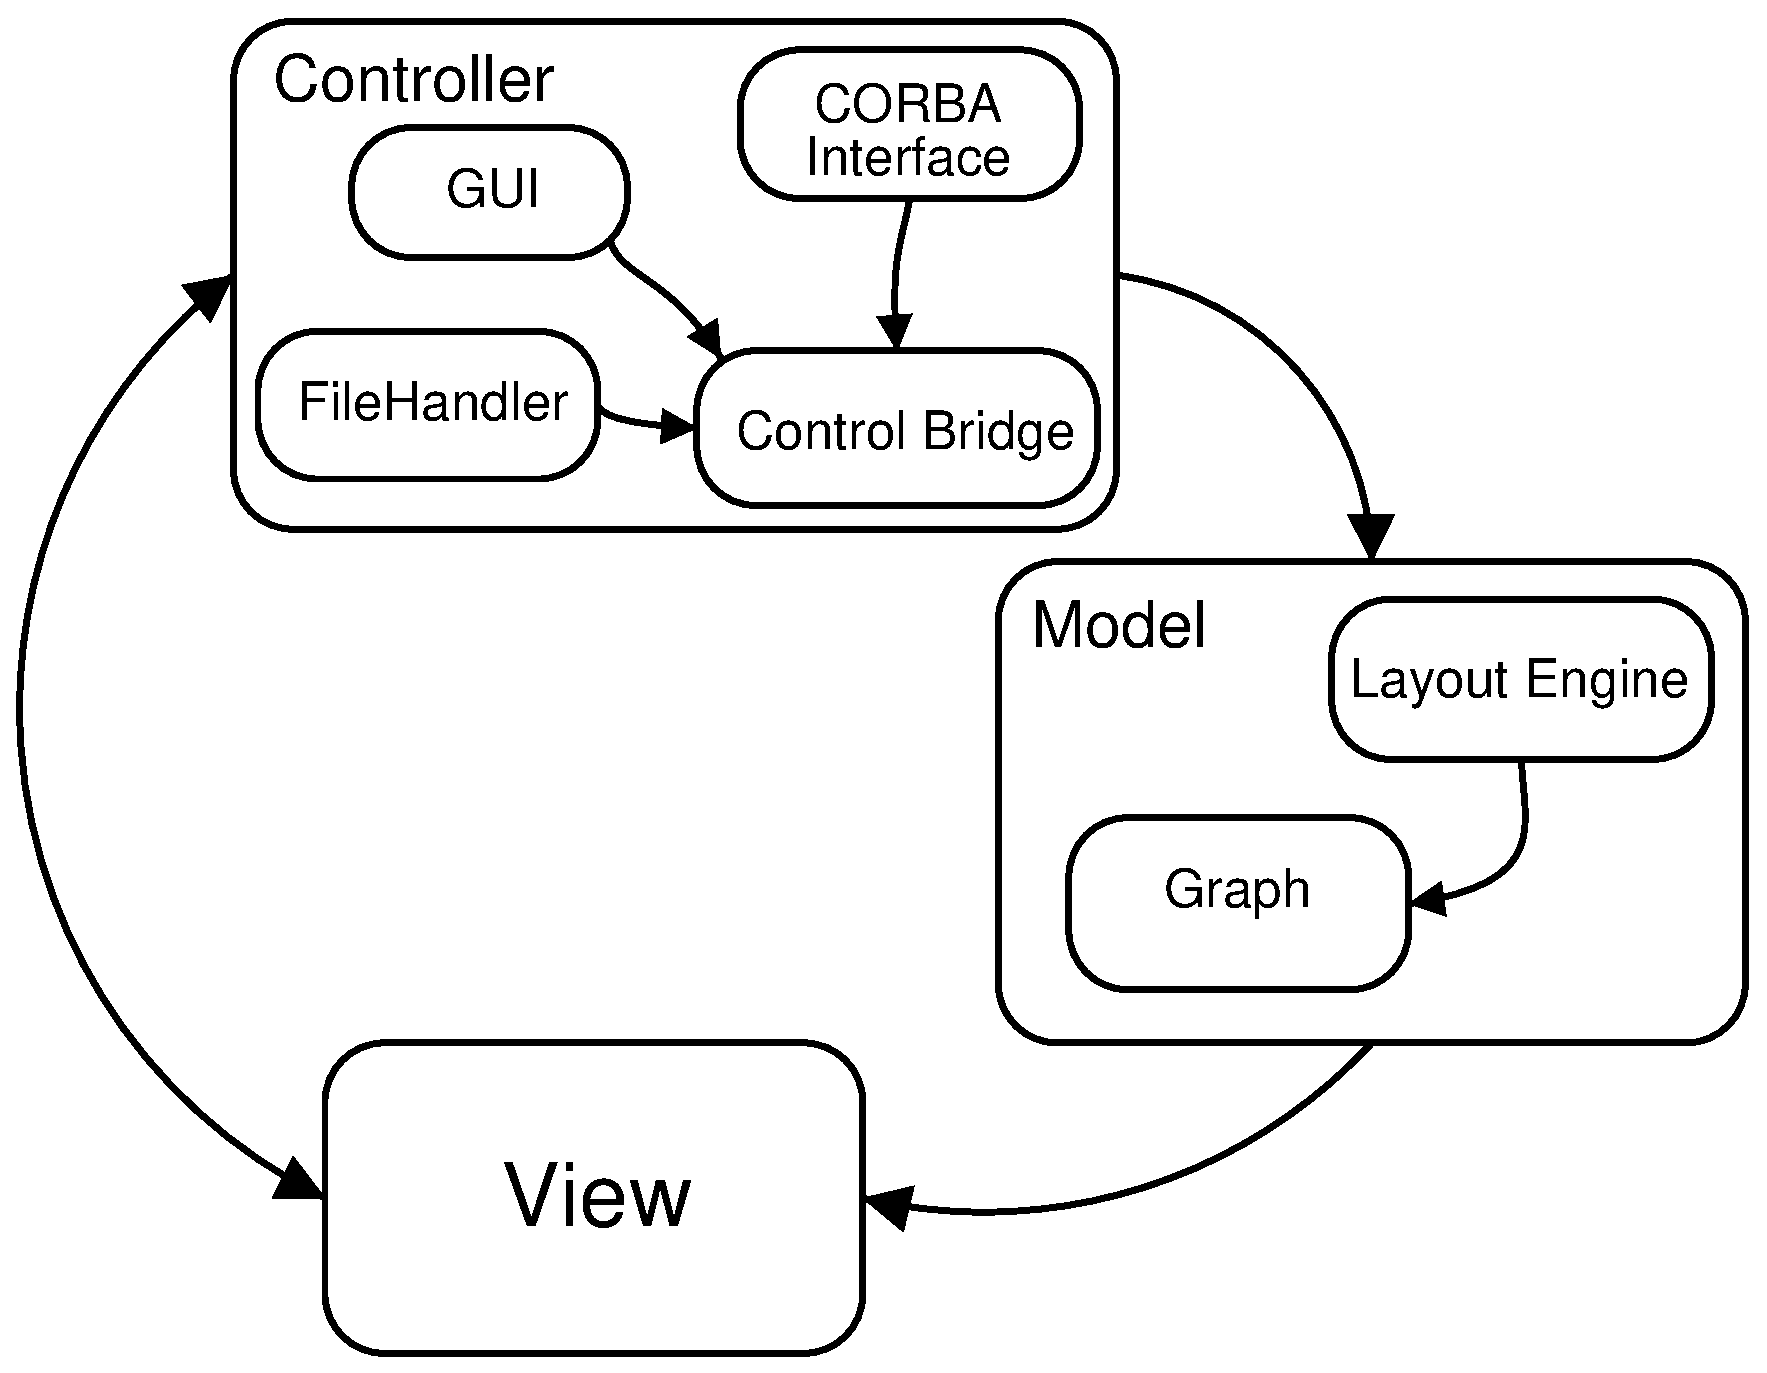
\includegraphics[width=0.5\textwidth]{figures/wilmamvc.eps}}
  \caption{The classic MVC framework and Wilma's utilisation of MVC.}
\end{figure}

In our system the Model is further broken down into two components:
the Graph data structure itself, capable of representing the structure
and state of the graph including its arrangement in space, and
the Layout Engine, which is an abstraction of the basic methods required for
an implementation of any layout algorithm that will change the graph's
arrangement in space.

A further requirement for our system is that the graph data model and
the layout engine should able to be controlled either interactively by
the user, by loading data from a file or even by remote
procedure call from a program running in another process or possibly on
another machine (Wilma's APIs are described in Section~\ref{API}).  Therefore the Controller component was also broken
down into several components.  A ``bridge'' layer provides a common
programmatic interface to the Model.  The methods provided by this
bridge layer can then be called by either the GUI interface component,
a component providing a CORBA interface for RPC or a component which
can load and save files to an XML format.


Figure \ref{fig-wilmamvc} depicts this expanded MVC architecture for graph
visualisation. 

\subsection{An Object-Oriented Graph Model}
In designing the Graph Model, ie, the data structures for storing the
graph and the methods for manipulating them, some common
elements were identified.  Firstly a graph consists fundamentally
of nodes and edges.  These are the basic Graph Elements.  A clustered
graph has nodes which may themselves be graphs, or clusters.

This description of a graph is modelled in a class hierarchy by
defining an abstract class {\em GraphElement} which is implemented by
both the {\em Node} and {\em Edge} classes.  A {Cluster} will inherit
all the properties of the {\em Node} class and also contains an
aggregation of {\em Nodes} and {\em Edges}.  A {Cluster} also contains
a reference to an abstract definition of a {\em LayoutEngine} which
provides a common interface to an implementation of a layout algorithm
for arranging the graph in 2 or 3 dimensional space.  Since the
details of the algorithm are kept separate it is easy to mix and match
different layout styles to different graphs or even clusters within
the one graph.  A similar class hierarchy was developed independantly
by Marshall et.  al\cite{marshall00object} around the same time.
Figure \ref{fig-wilmaclasses} shows a UML diagram depicting this
graph class hierarchy, and also shows how this relates to a force
directed {\em LayoutEngine} implementation, discussed further in
Section \ref{sec:forcedirectedlayout}.  In Figure
\ref{fig-wilmaclasses3d} we show a 3D
interpretation of this UML diagram rendered by Wilma in an application
of the system described further in \ref{sec:3duml}.

\begin{figure}[h]
  \centering
  \subfigure[UML Class diagram.]{
    \label{fig-wilmaclasses}
    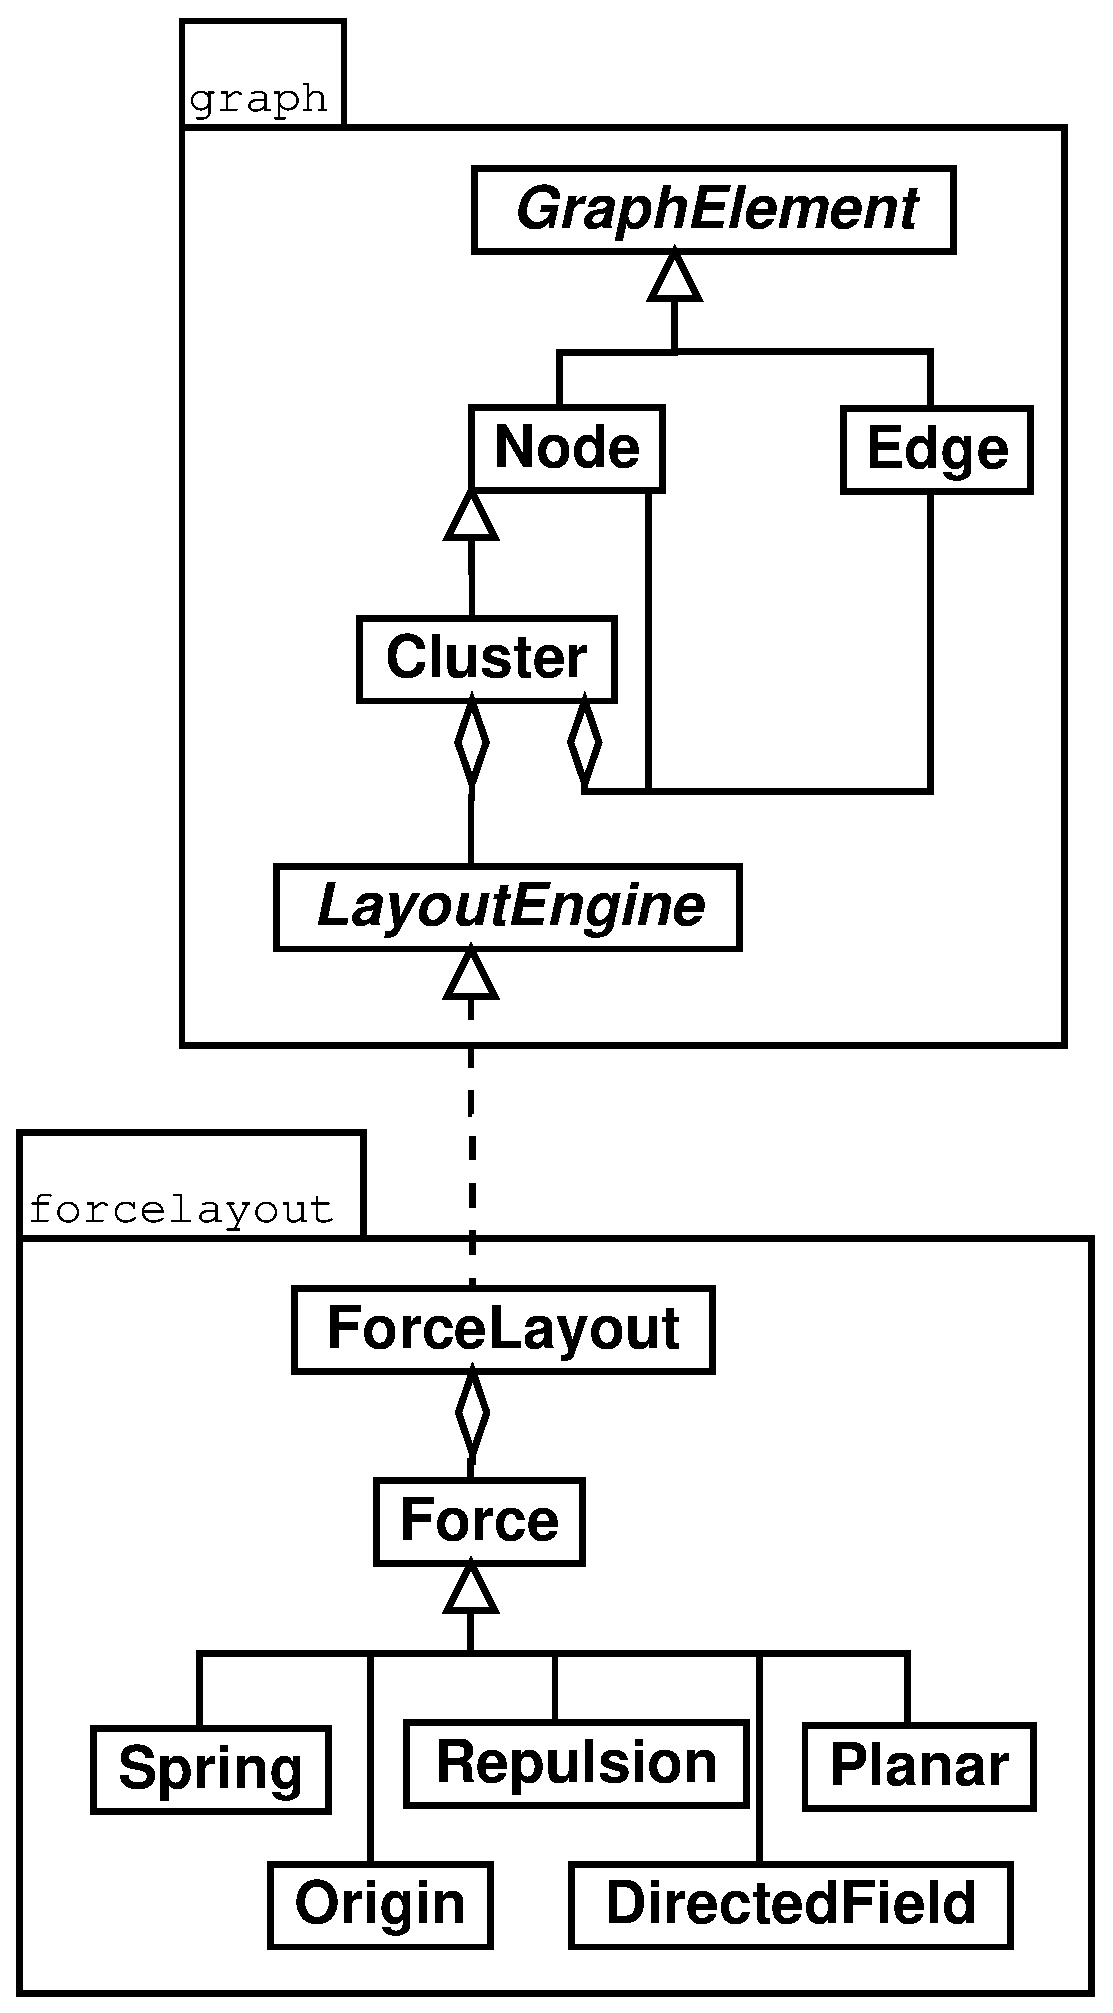
\includegraphics[width=0.35\textwidth]{figures/wilmaclasses.eps}}
  \subfigure[A 3D interpretation of the class hierarchy.]{
    \label{fig-wilmaclasses3D}
    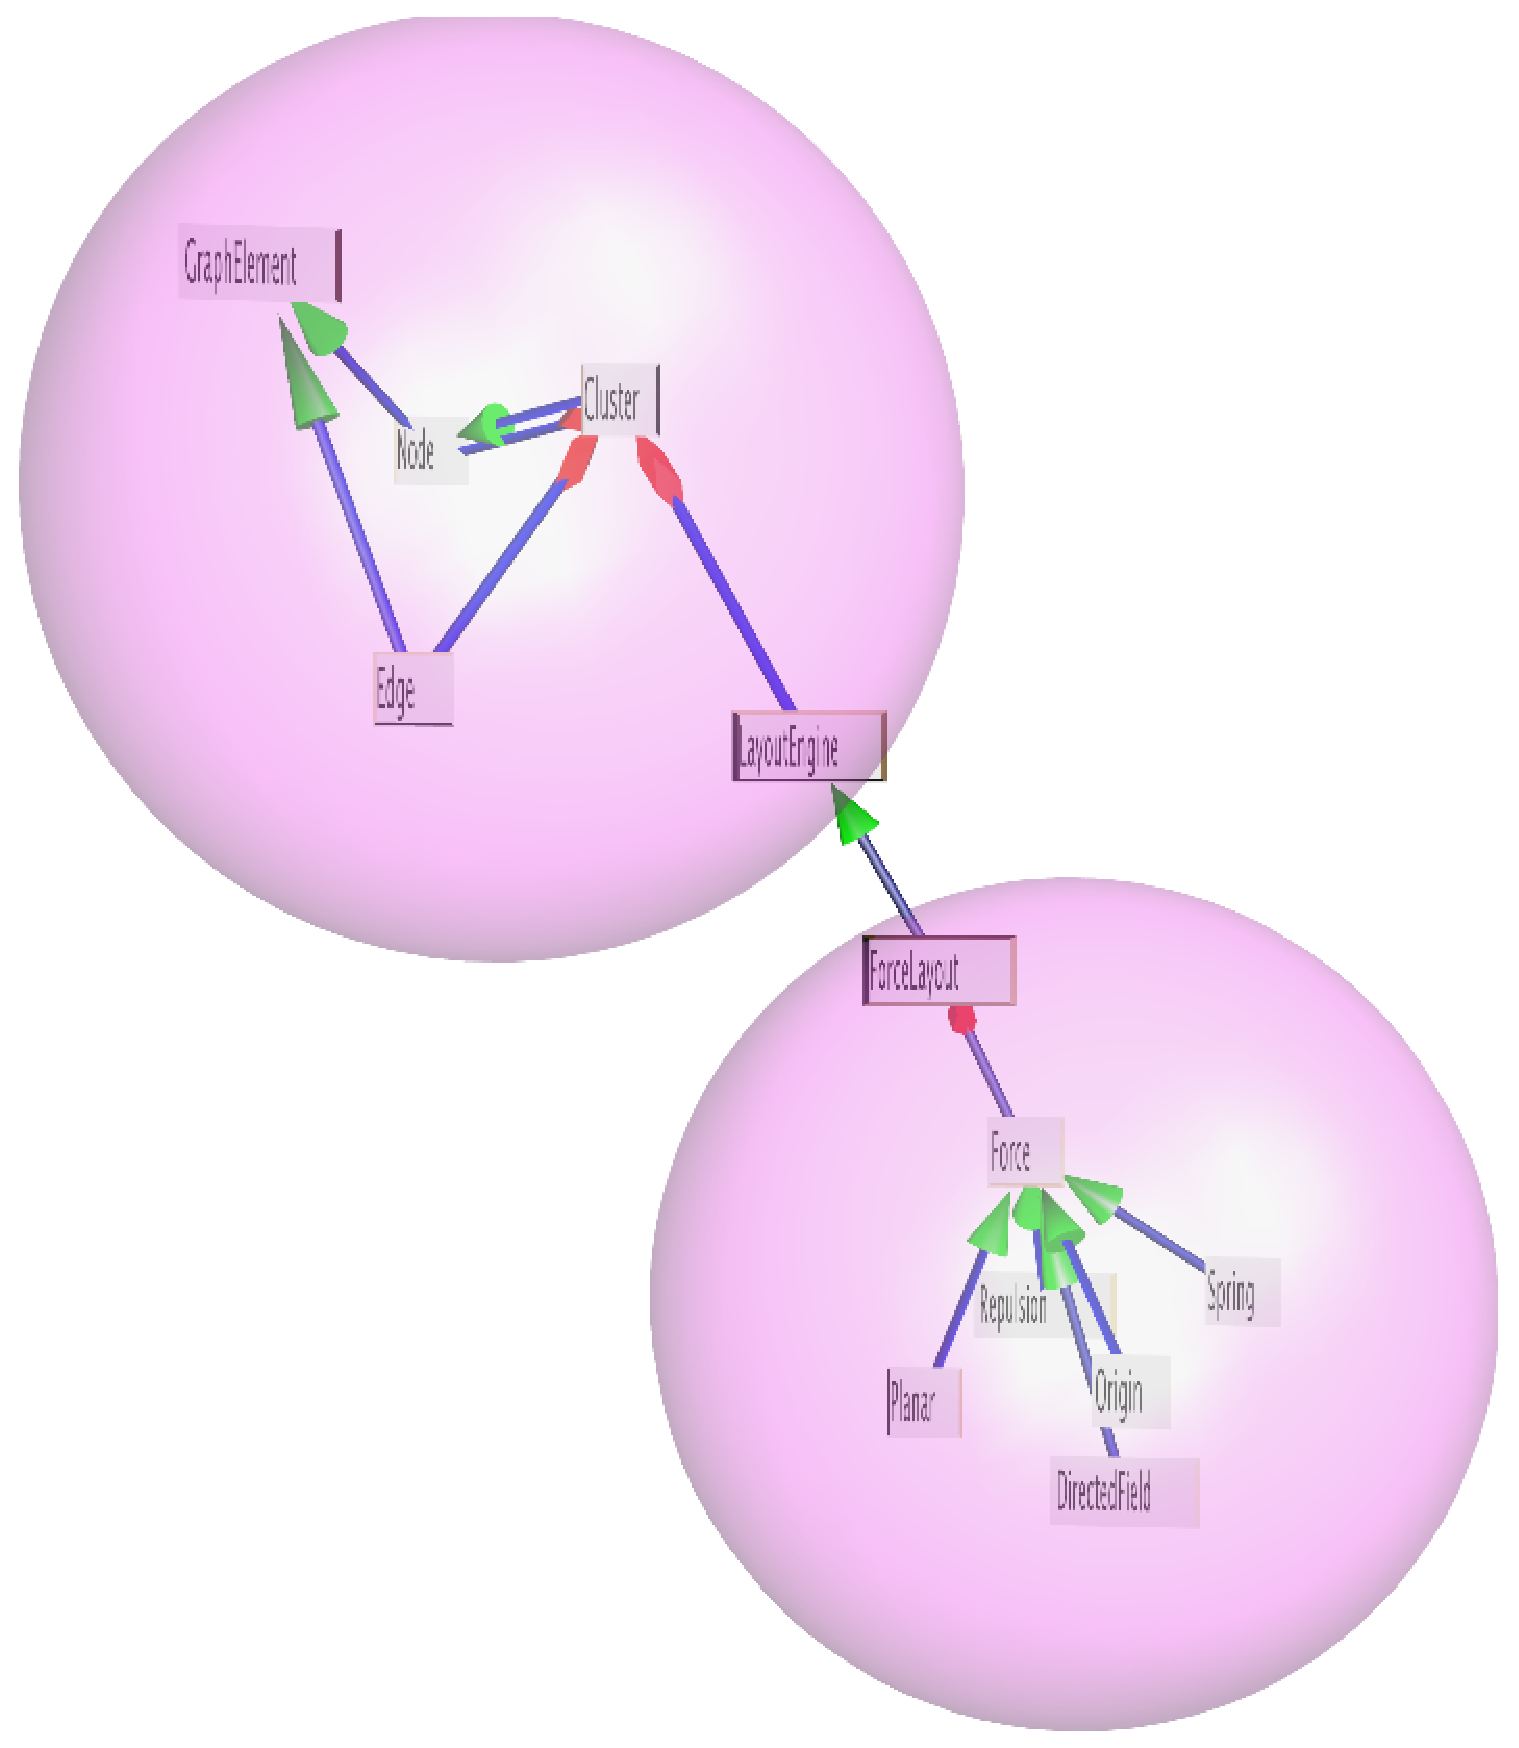
\includegraphics[width=0.55\textwidth]{figures/wilmaclasses3d.eps}}
  \caption{A class hierarchy for the graph model and the classes used
  in the Force Directed Layout Engine implementation.}
\end{figure}

\subsection{Layout Algorithms}
\subsubsection{Force Directed} \label{sec:forcedirectedlayout}
\subsubsection{Multiscale Force Directed}

\subsubsection{Fast Simulated Annealing}

As we stated in Section~\ref{motivation}, a major design goal for Wilma
was to provide a platform within which algorithmic experimentation could be
conducted elegantly and efficiently.

Force-directed layout algorithms are of course the method of choice for a
wide range of graph visualisation problems.  One variation on these
algorithms, advocated by Fruchtermann \&
Rheingold~\cite{fruchtermann90force-directed} and Davidson {\em et.
al.}~\cite{davidson01noise}, attempts to avoid calculation of repulsion force
vectors, which is $O(n^2)$ in the number of verticies:  

\begin{equation}
\vec{R}_i \equiv \sum_{j \in G, j \neq i} \vec{r}_{i,j}
\end{equation}

\noindent Where $\vec{r}_{i,j} = \vec{r}_i - \vec{r}_j$ is the displacement
of node $i$ relative to $j$.

To avoid this expense, it is possible to approximate scalar energy potential
values, caching this information at grid points throughout space.  Iterated
updates to the potential well then cost only $O(|V|)$ time per iteration.  On
the downside, the cache array itself takes $O(v \centerdot d)$ memory, where
$v$ is the $n$-dimensional volume (or area) of the embedded graph and $d$ is
the density of stored potential data points.

Cowling~\cite{cowling02fast} has implemented a fast layout engine for
WilmaScope which employs simulated annealing with potential energy caching
to achieve linear-time graph embeddings.  Cowling was able to demonstrate
that the algorithms of \cite{davidson01noise} do appear to achieve linear
time results, but that when the grid size $v \centerdot d$ must be adjusted to
prevent folding in large graphs, space and time complexity are
no longer linear.

Cowling's work serves to demonstrate the utility of Wilma as an empirical
platform; with the WilmaScope rendering and navigation system, and the
availability of convenient data structures for input and dataset management,
algorithmic experiments can be performed at optimal speeds.

\subsubsection{DOT: heirarchical layout}
\subsection{User Interfaces}
\subsection{Programming Interfaces}
\label{API}

A key design goal for Wilma was the provision of graph visualisation
facilities for other programs with very low barriers to development.  In order
to achieve this, we have implemented two external access APIs which give
programmers the ability to call up, extend and manipulate graph visualisations
in real-time.  These are the WilmaChat graph definition language, and the
Wilma CORBA interface.

\subsubsection{WilmaChat: A Dialogue on Graph Structure}

The simplest and lowest-energy programming interface to Wilma is the WilmaChat
language.  WilmaChat operates by creating a server daemon which listens on a
socket or pipe on the machine in question.

Clients can connect to WilmaChat and control graphs by passing commands
in a simple language which allows them to instantiate arbitrary graph
structures.

The advantage of WilmaChat is that it requires extremely little infrastructure
from the developers's programming environment.  The ability to traverse
internal graph structures and print a simple, formalised description of them
is enough to produce navigable 3D output.

\subsubsection{The Wilma CORBA Interface}

While the WilmaChat language is extremely efficient for rapid application
development, and can be driven by any programming environment on Wilma's
supported platforms, there are a number of advanced features for which the
socket dialogue is an inefficient mode of interaction.  For example, if
developers want multiple clients to connect to a particular Wilma server, in
the presence of access-control mediation; or if they wish to perform detailed
interrogation of the graph embedding which Wilma has created --- then the use
of a custom language requires more overhead.

In order to meet these more sophisticated requirements, we have implemented a
Wilma control interface which sits atop CORBA (the Common Object Request
Broker Archicture --- see \url{http://www.corba.org}).  Since CORBA provides
its own access control mechanisms, and good CORBA bindings handle all the
marshalling and type requirements for a sophisticated API, programmers using
languages which support CORBA can take advantage of these facilities without
writing additional code.

\section{Results: The Importance of being Wilma}
\label{sec:results}

\subsection{Applications}

\subsubsection{3D UML Visualisation} \label{sec:3duml}

Dwyer~\cite{dwyer013D-UML} has managed to obtain a peer-reviewed paper by
using Wilma to visualise UML structures for software engineering purposes.
Therefore, Wilma rocks.

\subsubsection{Web Structure Visualisation}

One early application of Wilma was to the representation of web structure, and
to visualising clustering algorithms for categorising such
structure\cite{eckersley2kclassiscope}.

An example of web structure visualisation is shown in Figure~\ref{fig-web}.
This is a dataset collected in 2000 from the website \url{www.linuxlinks.com}.
The clusters are defined over similarity between pages; also note the set of
17 pages (linked to every other page) which form site's navigation bar.

\begin{figure}
\begin{center}
\scalebox{0.8}{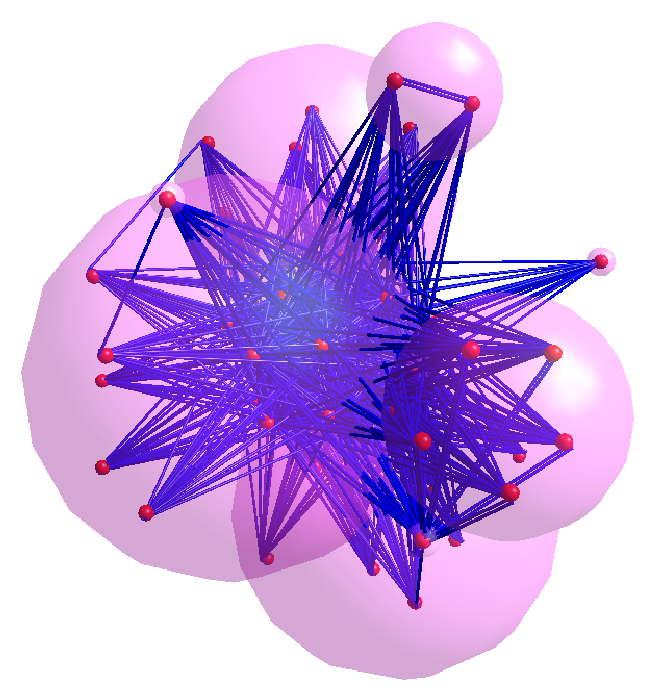
\includegraphics{figures/cluster1.eps}} \\
\caption{{\sc WilmaScope Visualisation of Web Site Structure}}
\label{fig-web}
\end{center}
\end{figure}

\begin{itemize}
\item pretty pictures
\item applications
\item self-congratulatory monologues
\end{itemize}

\section{Conclusions}
\label{sec:conclusions}
\begin{itemize}
\item megalomaniacal rants
\item further work
\item witty closing line
\end{itemize}

%\begin{thebibliography}{7}
%%
%\addcontentsline{toc}{section}{References}
%
%\bibitem{CHT93} Cai, J., Han, X., Tarjan, R.~E.\ (1993)
%An algorithm for the maximal planar subgraph
%problem.
%SIAM J.\ Comput.\ {\bf22}, 1142--1164
%
%\bibitem{DETT99} Di Battista, G., Eades, P., Tamassia, R., Tollis,
%  I.~G.\ (1999)
%Graph Drawing: Algorithms for the visualization of graphs.
%Prentice Hall, New Jersey
%
%\bibitem{Dji95} Djidjev, H.~N.\ (1995)
%A linear algorithm for the maximal planar subgraph problem.
%Proc.\ 4th Workshop Algorithms Data Struct., 
%Lecture Notes in Computer Science, Springer Verlag
%
%\bibitem{Eul1750} Euler, L.\ (1750)
%Demonstratio nonnullarum insignium proprietatum quibus solida hedris
%planis inclusa sunt praedita.
%Novi Comm.\ Acad.\ Sci.\ Imp.\ Petropol.\ {\bf4} (1752-3, published
%1758), 140--160, also: Opera Omnia (1) {\bf26}, 94--108
%
%\bibitem{KW01} Kaufmann, M., Wagner, D. (eds.) (2001)
%Drawing Graphs: Methods and Models.
%Lecture Notes in Computer Science 2025, Springer Verlag
%
%\bibitem{TDB88} Tamassia, R., Di Battista, G., Batini, C.\ (1988)
%Automatic graph drawing and readability of diagrams.
%IEEE Transactions on Systems, Man, and Cybernetics {\bf18}, 61--79
%
%\end{thebibliography}

\bibliographystyle{plain}
\newpage
\addcontentsline{toc}{section}{References}
\bibliography{refs}

%
%INDEX%%%%%%%%%%%%%%%%%%%%%%%%%%%%%%%%%%%%%%%%%%%%%%%%%%%%%%%%%%%%%%%
%\clearpage
%\addcontentsline{toc}{section}{Index}
%\flushbottom
%\printindex
%%%%%%%%%%%%%%%%%%%%%%%%%%%%%%%%%%%%%%%%%%%%%%%%%%%%%%%%%%%%%%%%%%%%%%

\end{document}
